% DOC SETTINGS ===================================
\documentclass{article}
\usepackage[utf8]{inputenc}
\usepackage{steinmetz}
\usepackage{mathtools}  
\usepackage{multicol}
\usepackage{circuitikz}
\usepackage{tikz}
\usepackage{listings}
\usepackage{geometry}
\usepackage{fancyhdr}
\usepackage{amsfonts}
\usepackage{media9}
\usepackage{parskip}
\usetikzlibrary{positioning, fit, calc}
\pagestyle{fancy}
\lhead{ECE2714 Problem Set 9}
\rhead{Kavin Thirukonda 2021}
\fancyheadoffset{0mm}
 \geometry{
 a4paper,
 total={170mm,257mm},
 left=20mm,
 top=25mm,
 }
\mathtoolsset{showonlyrefs} 
\cfoot{}
% DOC SETTINGS ===================================
\begin{document}
\begin{enumerate}
    \item Consider the time-domain signal
    \begin{equation}
        x(t) = \begin{cases}
        e^{5t} &  t < 0\\
        e^{-t} & t \geq 0
        \end{cases}
    \end{equation}
    \begin{enumerate}
        \item Find the Fourier transform of x(t) using the definition
        \begin{align}
            X(j\omega) &= \int_{-\infty}^\infty x(t) e^{-j\omega t}dt\\
            &= \int_{-\infty}^0 e^{5t} e^{-j\omega t}dt+\int_{0}^\infty e^{-t} e^{-j\omega t}dt\\
            &= \frac{1}{-j\omega +5}e^{-j\omega t+5t}\Bigg|_{-\infty}^0 + \frac{1}{-j\omega - 1}e^{-j\omega t-t}\Bigg|_{0}^\infty\\
            &= \frac{1}{-j\omega +5}(1-0) + \frac{1}{-j\omega - 1}(0-1)\\
            &= \boxed{\frac{1}{5 - j\omega } + \frac{1}{1 + j\omega}}
        \end{align}
        \item Plot the Magnitude and Phase Spectrum of the Signal from -20 to 20 radians per seconds
        \begin{align}
            |X(j\omega)| &= \frac{1}{5 - j\omega } + \frac{1}{1 + j\omega}\\
            &= \frac{1}{\sqrt{\omega^2+25}}+\frac{1}{\sqrt{\omega^2+1}}
        \end{align}
        \begin{align}
            \phase{X(j\omega)} &= \frac{1}{5 - j\omega } + \frac{1}{1 + j\omega}\\
            &= -\arctan(\frac{5}{-\omega}) + -\arctan(\frac{1}{\omega})\\
        \end{align}
        \begin{center}
            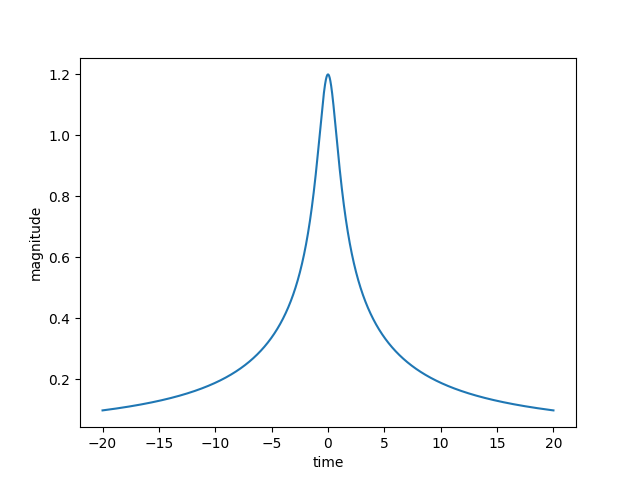
\includegraphics[width = .35\textwidth]{ps9_problem1b_mag.png}
            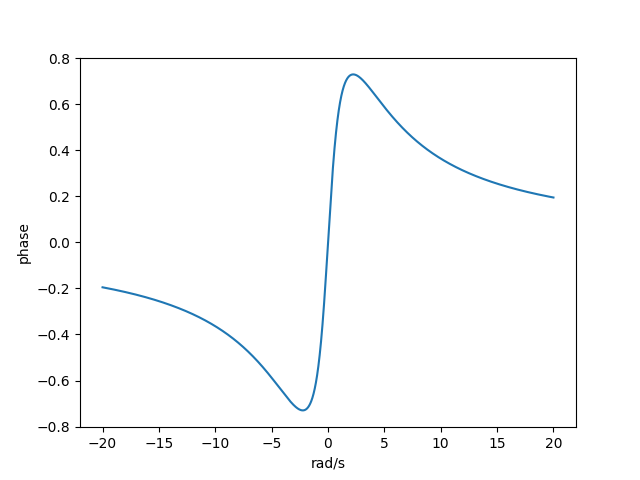
\includegraphics[width = .35\textwidth]{ps9_problem1b_phase.png}
        \end{center}
    \end{enumerate}
    \newpage
    \item Consider the signal represented in the frequency domain as
    \begin{equation}
        X(j\omega) = \frac{19+j6\omega}{18-\omega^2+j11\omega}
    \end{equation}
    \begin{enumerate}
        \item Write the signal in the form
        \begin{equation}
            X(j\omega) = \frac{A}{2+j\omega}+\frac{B}{9+j\omega}
        \end{equation}
        i.e. determine the constants A and B
        \begin{align}
            &X(j\omega) = \frac{19+j6\omega}{18-\omega^2+j11\omega}\\
            &\Rightarrow X(j\omega) = \frac{19+j6\omega}{(2+j\omega)(9+j\omega)}\\
            &\Rightarrow \frac{19+j6\omega}{18-\omega^2+j11\omega} = \frac{A}{2+j\omega}+\frac{B}{9+j\omega}\\
            &\Rightarrow 19+j6\omega = A(9+j\omega)+B(2+j\omega)\bigg|_{\omega = -j9, -j2}\\
            &\Rightarrow 73 = A(18)+B(11)\\
            &\Rightarrow 31 = A(11)+B(4)\\
            &\Rightarrow \boxed{A = 1, B = 5}
        \end{align}
        \item Using your result from part a) find the signal representation in the time-domain i.e. x(t)
        \begin{align}
        X(j\omega) &= \frac{1}{2+j\omega}+\frac{5}{9+j\omega}\\
        &= \boxed{(e^{-2t}+5e^{-9t})u(t)}
        \end{align}
    \end{enumerate}
    \newpage
    \item Consider the continuous-time rectangular pulse signal, x(t), given by the expression,
    \begin{equation}
        x(t) = \begin{cases}
        1, & -a < t < a \\
        0, & else
        \end{cases}
    \end{equation}
    Determine the continuous-time Fourier transform $X(\omega)$ from the definition.
    \begin{align}
        X(j\omega) &= \int_{-\infty}^\infty x(t) e^{-j\omega t}dt\\
        &= \int_{-a}^a e^{-j\omega t}dt\\
        &= -\frac{1}{j\omega} e^{-j\omega t}\bigg|_{-a}^a\\
        &= -\frac{1}{j\omega} (e^{-j\omega a}-e^{j\omega a})\\
        &= \frac{1}{j\omega} (e^{j\omega a}-e^{-j\omega a})\\
        &= \frac{1}{j\omega} (j\sin(\omega a))\\
        &= \boxed{\frac{2\sin(\omega a)}{\omega}}
    \end{align}
    \newpage
    \item Consider the discrete-time rectangular pulse signal, x[n], given by the expression,
    \begin{equation}
        x[n] = u[n] -u[n-N].
    \end{equation}
    Determine the discrete-time Fourier transform $X(e^{j\omega})$ from the definition.
    \begin{align}
        X(e^{j\omega}) &= \sum_{n=-\infty}^\infty x[n]e^{-j\omega n}\\
        &= \sum_{n=0}^N e^{-j\omega n}\\
        &= \sum_{n=0}^{N-     1} (e^{-j\omega})^n\\
        &= \boxed{\frac{1-e^{-j\omega(N+1)}}{1-e^{-j\omega}}}
    \end{align}
    \newpage
    \item Consider the  continuous time signal, y(t), given by the expression,
    \begin{equation}
        y(t) = x(t)cos(\omega_ot)
    \end{equation}
    where
    \begin{equation}
        x(t) = \begin{cases}
        1 & |t| < T\\
        0 & else
        \end{cases}
    \end{equation}
    Determine the Fourier Transform, $Y(j\omega)$ of y(t) using the multiplication property of the Fourier Transform.
    \begin{align}
        X(j\omega) &= \int_{-\infty}^\infty x(t)e^{-j\omega t}dt\\
        &= \int_{-T}^T e^{-j\omega t}dt\\
        &= \frac{1}{j\omega}e^{-j\omega t}\bigg|_{-T}^T\\
        &= \frac{1}{j\omega}\left(e^{-j\omega T}-e^{j\omega T}\right)\\
        &= \frac{2\sin(\omega T)}{\omega}\bigg|_{X(0)=2T}
    \end{align}
    \begin{align}
        C(j\omega) &= \int_{-\infty}^\infty\cos(\omega_ot)e^{-j\omega t}dt\\
        &= \int_{-\infty}^\infty\frac{1}{2}e^{j\omega t}e^{-j\omega t}dt -\int_{-\infty}^\infty\frac{1}{2}e^{-j\omega t}e^{-j\omega t}dt\\
        &= \frac{1}{2}(2\pi\delta(\omega-\omega_o)+2\pi\delta(\omega+\omega_o))\\
        &= \pi(\delta(\omega-\omega_o)+\delta(\omega+\omega_o))
    \end{align}
    \begin{align}
        Y(j\omega) &= \frac{1}{2\pi}X(j\omega)*C(j\omega)\\
        &= \frac{1}{2\pi}(\frac{2\sin(\omega T)}{\omega})*\pi(\delta(\omega-\omega_o)+\delta(\omega+\omega_o))\\
        &= (\frac{\sin(\omega T)}{\omega})*(\delta(\omega-\omega_o)+\delta(\omega+\omega_o))\\
        &= (\frac{\sin(\omega T)}{\omega})*(\delta(\omega-\omega_o))+(\frac{\sin(\omega T)}{\omega})*(\delta(\omega+\omega_o))\\
        &= \boxed{\frac{\sin((\omega-\omega_o) T)}{(\omega-\omega_o)}+\frac{\sin((\omega+\omega_o) T)}{(\omega+\omega_o)}}
    \end{align}
    \newpage
    \item Consider the discrete time signal, x[n], given by the expresion,
    \begin{equation}
        x[n] = a^nu[n] 
    \end{equation}
    where $|a| < 1$.
    \begin{enumerate}
        \item Determine the Discrete Time Fourier Transform, $X(e^{j\omega})$ of x[n] using the definition of the Discrete Time Fourier Transform.
        \begin{align}
            X(e^{j\omega}) &= \sum_{n=-\infty}^\infty x[n]e^{-j\omega n}\\
            &= \sum_{n=0}^\infty a^ne^{-j\omega n}\\
            &= \sum_{n=0}^\infty (ae^{-j\omega})^n\\
            &= \boxed{\frac{1}{1-ae^{-j\omega}}}
        \end{align}
        \item Create an expression for $|X(e^{j\omega})|$ (magnitude spectrum). Simplify as much as possible.
        \begin{align}
            |X(e^{j\omega})| &= \frac{|1|}{|1-ae^{-j\omega}|}\\
            &= \frac{1}{\sqrt{(1-a\cos(\omega))^2+(aj\sin(\omega))^2}}\\
            &= \frac{1}{\sqrt{a^2\cos^2(\omega)-2a\cos(\omega)+1+a^2\sin^2(\omega)}}\\
            &= \frac{1}{\sqrt{a^2(\cos^2(\omega)+\sin^2(\omega))-2a\cos(\omega)+1}}\\
            &= \boxed{\frac{1}{\sqrt{a^2-2a\cos(\omega)+1}}}
        \end{align}
        
        \item Create an expression for $\phase{X(e^{j\omega})}$ (phase spectrum). Simplify as much as possible.
        \begin{align}
            \phase{X(e^{j\omega})} &= \phase{1}-\phase{1-ae^{-j\omega}}\\
            &= 0-\phase{1-a(\cos(\omega)-j\sin(\omega))}\\
            &= \boxed{-\tan^{-1}\left(\frac{1-a\cos(\omega)}{a\sin(\omega)}\right)}
        \end{align}
    \end{enumerate}
\end{enumerate}
\end{document}
